\chapter*{Übung 5}

\section*{Aufgabe 11}

Siehe Abbildung \ref{fig:ueb5_aufgabe11} für eine Skizze mit den Variablen.

\begin{figure}[h]
	\centering
	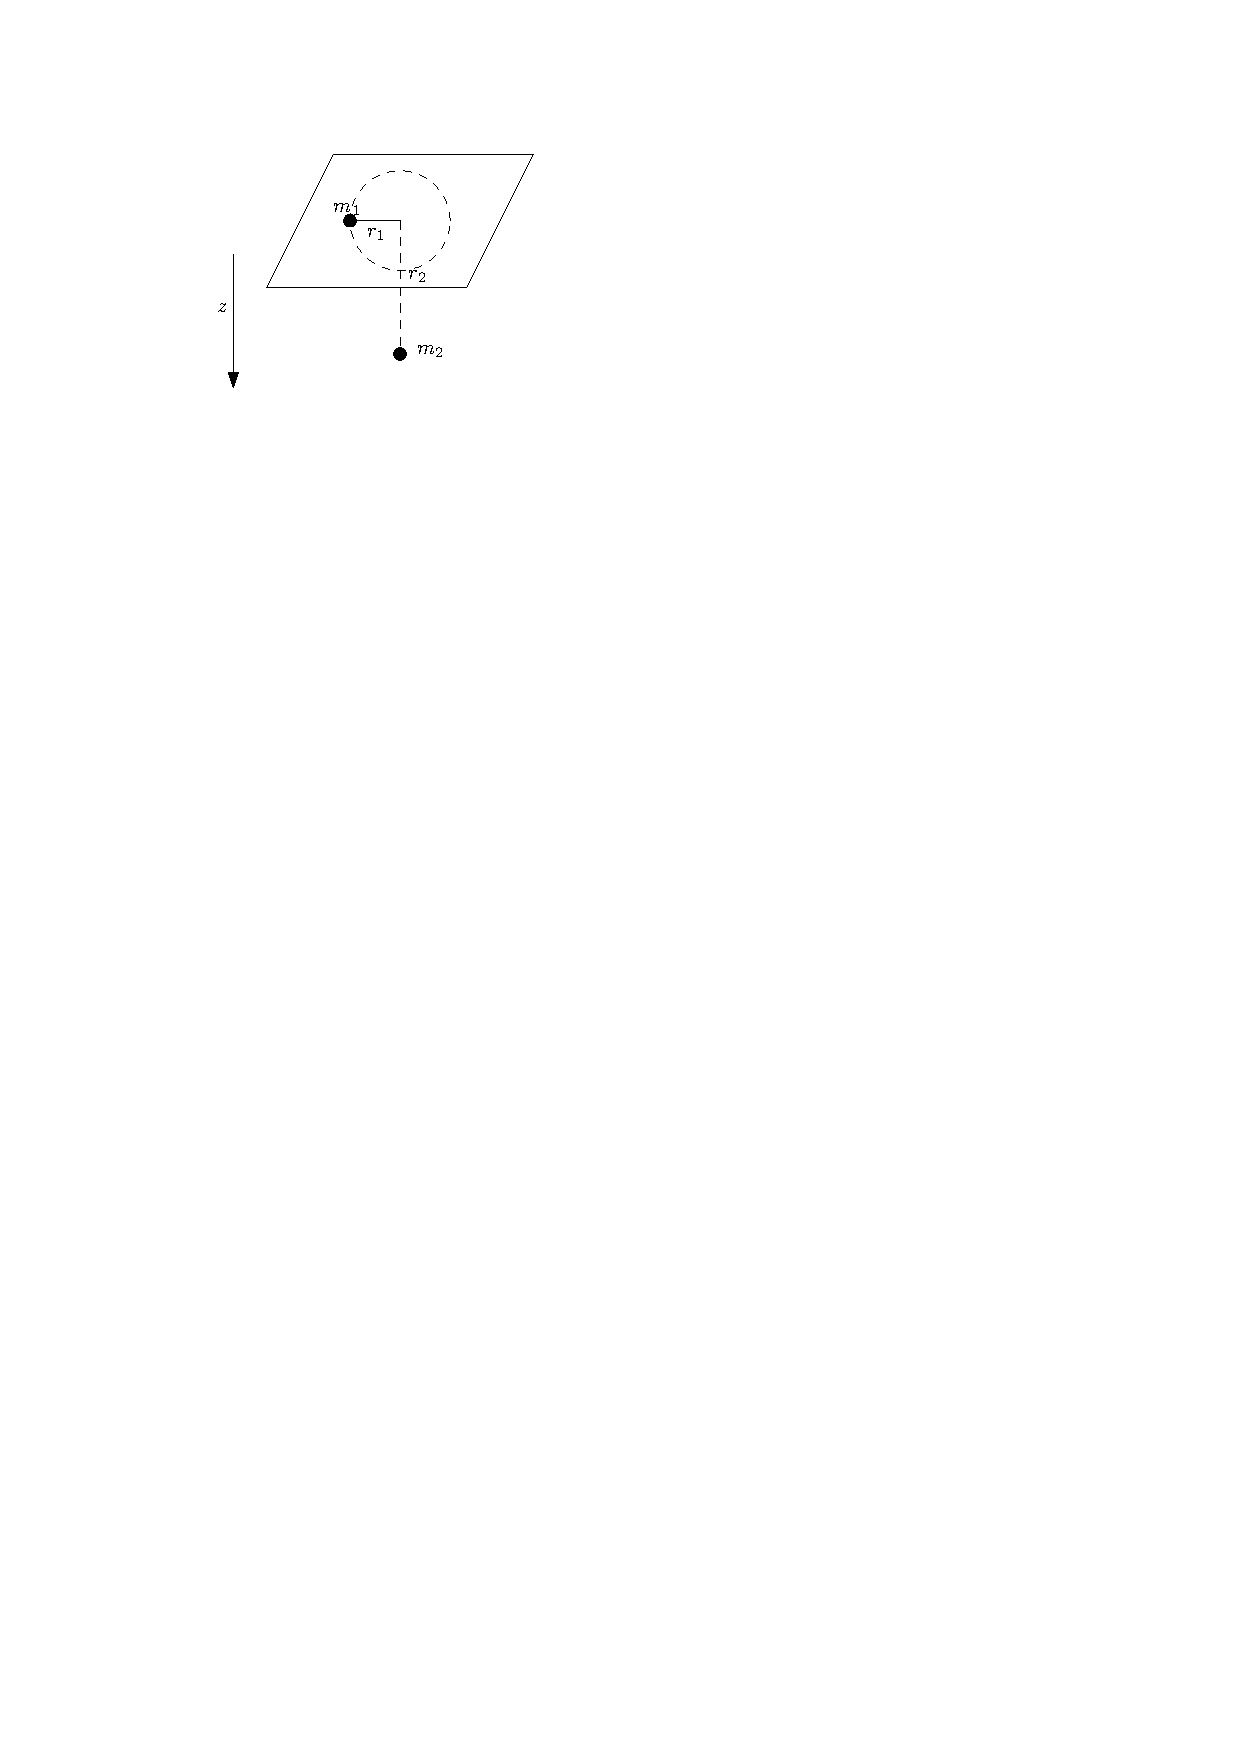
\includegraphics{figures/ueb5/aufgabe11}
	\label{fig:ueb5_aufgabe11}
	\caption{Skizze von Aufgabe 11. Die Koordinate $z$ zeigt nach unten.}
\end{figure}

Wir wählen als Koordinaten:
\[
	\vec{x}_1 = \mvec{ \cos \phi_1 r_1 \\ \sin \phi_1 r_1 \\ z_1} 
	\quad \text{ und } \quad 
	\vec{x}_2 = r_2 \mvec{ \sin \theta_2 \cos \phi_2 \\ \sin \theta_2 \sin \phi_2 \\ \cos \theta_2 }
	\text{.}
\]

Also $F_g = m g \vec{e}_z = - \vec{\nabla} V_g$ mit $V_g = - m g z$ (auf Vorzeichen achten).

Die Länge vom Seil ist $l = r_1 + r_2$. Also Zwangsbedingung: $A = r_1 + r_2 - l = 0$ und $z_1 = const$. Wähle $z_1 = 0$, dann: $V_{g, 1} = - m_1 g \cdot 0 = 0$.

Damit ist $T_1 = \frac{1}{2} m_1 (\dot{x}_1^2 + \dot{y}_1^2)$, wobei 
\begin{align*}
	\dot{x}_1 &= \dot{r}_1 \cos \phi_1 - r_1 \dot{\phi}_1 \sin \phi_1 \text{ und} \\
	\dot{y}_1 &= \dot{r}_1 \sin \phi_1 + r_1 \dot{\phi}_1 \cos \phi_1 
	\text{.}	
\end{align*}

Also eingesetzt (Rechnung analog zu Aufgabe 10): $T_1 = \frac{1}{2} m_1 \left( \dot{r}_1^2 + r_1^2 \dot{\phi}_1^2 \right)$. Weiterhin 
\[
	T_2 \overset{\text{Aufg. 10}}{=} \frac{1}{2} m_2 \left( \dot{r}_1^2 + r_2^2 \dot{\theta})_2^2 + r_2^2 \dot{\phi}_2^2 \sin^2 \theta_2 \right)
	\text{.}
\]

Ingesamt folgt die Lagrange-Funktion, wobei $r_2 = l - r_1$ und $\dot{r}_2 = \dot{r}_1$ genutzt wird:
\begin{align*}
	L 
	&= T_1 + T_2 - V_1 - V_2 \\
	&= \frac{1}{2} m_1 \left( \dot{r}_1^2 + r_1^2 \dot{\phi}_1^2 \right)
	+ \frac{1}{2} m_2 \left( \dot{r}_2^2 + r_2 ^2 \dot{\theta}_2^2 + r_2^2 \dot{\phi}_2^2 \sin^2 \theta_2 \right)
	+ m g r_2 \cos \theta_2 \\
	&= \frac{1}{2} (m_1 + m_2) \dot{r}_1^2 
	+ \frac{1}{2} m_1 r_1^2 \dot{\phi}_1^2
	+ \frac{1}{2} (l - r_1)^2 (\dot{\theta}_2^2 + \dot{\phi}_2^2 \sin^2 \theta_2)
	+ m_2 g (l - r_1) \cos \theta_2
	\text{.}
\end{align*}

Was sind die zyklischen Koordinaten? Die müssen die Bedingung
\[
	\frac{\partial L}{\partial q_i} = 0 
	\quad \text{ und } \quad 
	\frac{\partial L}{\partial \dot{q}_i} \neq 0
\]
erfüllen.

Erhalten sind 
\begin{align*}
	P \phi_1 &= \frac{\partial L}{\partial \dot{\phi}_1} = m_1 r_1^2 \dot{\phi}_1 \text{ und } \\
	P \phi_2 &= \frac{\partial L}{\partial \dot{\phi}_2} = m_2 (l - r_1)^2 \sin^2 \theta_2 \dot{\phi}_2
	\text{.}
\end{align*}

Jetzt Einschränkung: $\phi_2 = \theta_2 = 0$. Damit vereinfacht sich die Lagrange-Funktion zu 
\[
	L = \frac{1}{2} (m_1 + m_2) \dot{r}_1^2 + \frac{1}{2} m_1 r_1^2 \dot{\phi}_1^2 + m_2 g (l - r_1) = L(r_1, \phi_1)
	\text{.}
\]	
Damit bestimmen wir die Lagrange-Gleichungen:
\begin{align*}
	& \frac{\partial L}{\partial r_1} = \msimplediff{}{t} \frac{\partial L}{\partial \dot{r}_1} \\
	\Longrightarrow~ & m_1 r_1 \dot{\phi}_1^2 - m_2 g = \msimplediff{}{t} \left( (m_1 + m_2) \dot{r}_1 \right) = (m_1 + m_2) \ddot{r}_1 \\
	\Longrightarrow~ & \ddot{r}_1 = \frac{1}{m_1 + m_2} \left( m_1 r_1 \dot{\phi}_1^2 - m_2 g \right) \\
	& \frac{\partial L}{\partial \phi_1} = \msimplediff{}{t} \frac{\partial L}{\partial \dot{\phi}} \\
	\Longrightarrow~ & 0 = \msimplediff{}{t} \left( m_1 r_1^2 \dot{\phi}_1 \right) = 2 m_1 \dot{r}_1 r_1 \dot{\phi}_1 + m_1 r_1^2 \ddot{\phi}_1 \\
	\Longrightarrow~ & \ddot{\phi}_1 = - \frac{2}{r_1} \dot{r}_1 \dot{\phi}_1
	\text{.}
\end{align*}

\section*{Aufgabe 12}

Für eine Skizze mit den Variablen siehe Abbildung \ref{fig:ueb5_aufgabe12}.

\begin{figure}
	\centering
	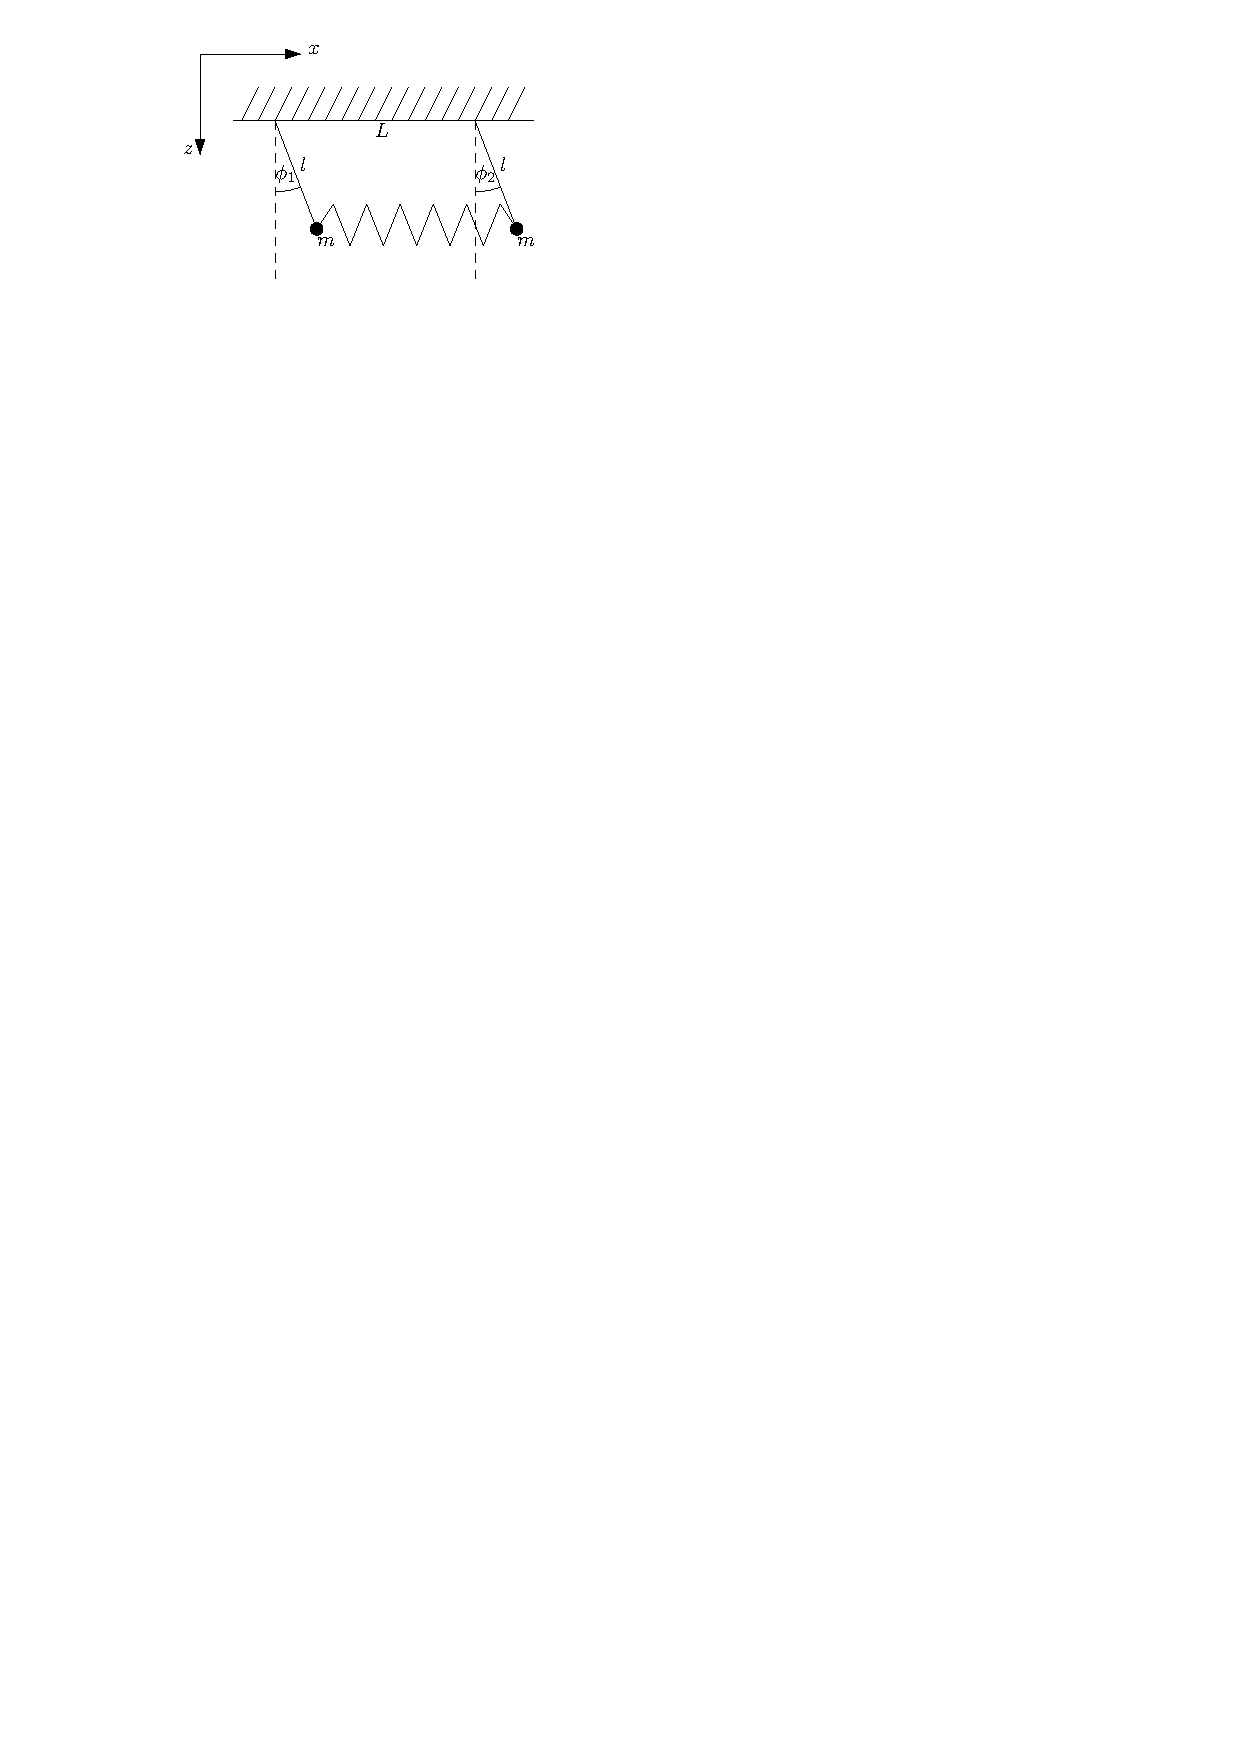
\includegraphics{figures/ueb5/aufgabe12}
	\label{fig:ueb5_aufgabe12}
	\caption{Skizze von Aufgabe 12.}
\end{figure}

Es gilt also:
\[
	x_1 = l \sin \phi_1,
	\quad 
	z_1 = l \cos \phi_1,
	\quad 
	x_2 = l \sin \phi_2 + L
	\quad \text{ und } \quad 
	z_2 = l \cos \phi_2
	\text{.}
\]

Damit folgen die Ableitungen
\begin{align*}
	\dot{x}_1 &= \dot{\phi}_1 l \cos \phi_1, \\
	\dot{x}_2 &= \dot{\phi}_2 l \cos \phi_2, \\
	\dot{z}_1 &= - l \dot{\phi}_1 \sin \phi_1 \text{ und } \\
	\dot{z}_2 &= - l \dot{\phi}_2 \sin \phi_2
	\text{.}
\end{align*}

Die Energien sind
\begin{align*}
	T &= \frac{1}{2} m \left( \dot{x}_1^2 + \dot{z}_1^2 \right)
	+ \frac{1}{2} m \left( \dot{x}_2^2 + \dot{z}_2^2 \right)	
	= \frac{1}{2} m l^2 \left( \dot{\phi}_1^2 + \dot{\phi}_2^2 \right), \\
	V_g &= \sum_{i = 1, 2} - m g z_i = - m g l (\cos \phi_1 + \cos \phi_2) \text{ und } \\
	V_F &= \frac{1}{2} \kappa (x_1 - (x_2 - L))^2 = \frac{1}{2} \kappa l^2 (\sin \phi_1 - \sin \phi_2)^2
\end{align*}
und die Lagrange-Funktion damit
\[
	L = \frac{1}{2} m l^2 (\dot{\phi}_1^2 + \dot{\phi}_2^2)
	- \frac{1}{2} \kappa l^2 (\sin \phi_1 - \sin \phi_2)^2
	+ m g l (\cos \phi_1 + \cos \phi_2)
	\text{.}
\]

Für kleine Auslenkungen approximieren wir mit Taylor:
\begin{align*}
	\sin(x) &= x + \mathcal{O}(x^2) \text{ und } \\
	\cos(x) &= 1 - \frac{x^2}{2} + \mathcal{O}(x^3) = 1 + \mathcal{O}(x^2)
	\text{.}
\end{align*}

Damit vereinfacht sich die Lagrange-Funktion zu
\[
	L = \frac{1}{2} m l^2 (\dot{\phi}_1^2 + \dot{\phi}_2^2)
	- \frac{1}{2} \kappa (\phi_1 - \phi_2)^2
	+ m g l \left( 2 - \frac{\phi_1^2}{2} - \frac{\phi_2^2}{2} \right)
	\text{.}
\]

Jetzt wieder die Lagrange-Gleichungen aufstellen:
\begin{align*}
	\msimplediff{}{t} \frac{\partial L}{\partial \dot{\phi}_1} &= m l^2 \ddot{\phi}_1, \\
	\msimplediff{}{t} \frac{\partial L}{\partial \dot{\phi}_2} &= m l^2 \ddot{\phi}_2, \\
	\frac{\partial L}{\partial \phi_1} &= - \kappa l^2 (\phi_1 - \phi_2) - m g l \phi_1 \text{ und } \\
	\frac{\partial L}{\partial \phi_2} &= \kappa l^2 (\phi_1 - \phi_2) - m g l \phi_2
	\text{.}
\end{align*}

Es folgen daraus die Differentialgleichungen
\[
	\ddot{\phi}_1 = - \frac{\kappa}{m} (\phi_1 - \phi_2) - \frac{g}{l} \phi_1
	\quad \text{ und } \quad 
	\ddot{\phi}_2 = \frac{\kappa}{m} (\phi_1 - \phi_2) - \frac{g}{l} \phi_2
	\text{.}
\]

Mit dem Hinweis:
\begin{align*}
	\ddot{\phi}_2 - \ddot{\phi}_1 &= 2 \frac{\kappa}{m} (\phi_2 - \phi_1) - \frac{g}{l} (\phi_2 - \phi_1), \\
	\underbrace{(\dot{\phi}_2 - \dot{\phi}_1)}_{= \dot{\Phi}_1} &= \left( 2 \frac{\kappa}{m} - \frac{g}{l} \right) \underbrace{\left( \phi_2 - \phi_1 \right)}_{= \Phi_1} \text{ und } \\
	\underbrace{(\dot{\phi}_1 + \dot{\phi}_2)}_{= \dot{\Phi}_2} &= - \frac{g}{l} \underbrace{(\phi_1 + \phi_2)}_{= \Phi_2} \text{.}
\end{align*}

\begin{description}
	\item[Gleichschwingung] $\phi_2 = \phi_1$ $\Longrightarrow$ $\Phi_1 = 0$
	\item[Gegenschwingung] $\phi_2 = -\phi_1$ $\Longrightarrow$ $\Phi_2 = 0$ 
\end{description}

Nun ans Lösen: Wähle den Ansatz 
\[
	\Phi_1(t) = A_1 \cos (\omega_1 t + \beta_1) 
	\quad \text{ und } \quad 
	\Phi_2(t) = A_2 \cos (\omega_2 t + \beta_2)
	\text{.}
\]

Das impliziert $\omega_1^2 = \frac{g}{l} - 2 \frac{\kappa}{m} = \frac{g}{l} \left( 1 - 2 \frac{\kappa}{g} \frac{l}{m} \right)$ und weiter $\omega_2^2 = \frac{g}{l}$. Die anderen Unbekannten bestimmen wir mit den Anfangsbedingungen:
\[
	\phi_1(t = 0) = A
	\quad \text{ und } \quad 
	\phi_2(t = 0) = 0
	\text{.}
\]

Damit $\Phi_1(t = 0) = \phi_1(t = 0) = -A$ und $\Phi_2(t = 0) = - \phi_2(t = 0) = A$. Weiter mit der Anfangsbedingung $\dot{\phi}_1(t = 0) = \dot{\phi}_2(t = 0) = 0$: 
\begin{align*}
	\dot{\Phi}_1(t = 0) &= 0 
	= - A_1 \omega_1 \sin (\omega_1 \cdot 0 + \beta_1) 
	= - A_1 \omega_1 \sin(\beta_1) \text{ und } \\
	\dot{\Phi}_2(t = 0) &= 0 
	= -A_2 \omega_2 \sin(\beta_2) \text{.}
\end{align*}
Also $\beta_1 = \beta_2 = 0$. Zuletzt $\ddot{\Phi}_1(t = 0) = A_1 = A$ und $\ddot{\Phi}_2(t = 0) = A_2 = A$ (wirklich $\ddot{\Phi}$?) 

Am Ende soll folgen: 
\[
	\Phi_1(t) = A \cos (\omega_1 t) 
	\quad \text{ und } \quad 
	\Phi_2(t) = A \cos (\omega_2 t)
	\text{.}
\]

Ergebnis:
\begin{align*}
	\phi_1(t) &= \frac{1}{2} (- \Phi_1 + \Phi_2) = \frac{1}{2} A (\cos(\omega_2 t) - \cos(\omega_1 t)) \text{ und } \\
	\phi_2(t) &= \frac{1}{2} (\Phi_1 + \Phi_2) = \frac{1}{2} A (\cos(\omega_1 t) + \cos (\omega_2 t))
	\text{.}
\end{align*}

Darauf kann man noch die Additionstheoreme $\cos x + \cos y = 2 \cos \left( \frac{x + y}{2} \right) \cos \left( \frac{x - y}{2} \right)$ und $\cos x - \cos y = - 2 \sin \left( \frac{x + y}{2} \right) \sin \left( \frac{x - y}{2} \right)$ anwenden:
\begin{align*}
	\phi_2(t) &= A \cos \left( \frac{\omega_1 + \omega_2}{2} t \right) \cos \left( \frac{\omega_2 - \omega_1}{2} t \right) \\
	\phi_1(t) &= - \underbrace{A \sin \left( \frac{\omega_1 + \omega_2}{2} t \right)}_{= A(t)} \sin \left( \frac{\omega_2 - \omega_1}{2} t \right)
\end{align*}

Interpretation: Die Amplitude ist auch von der Zeit abhängig; wenn die Amplitude von $\phi_2$ am größten ist, ist die Amplitude von $\phi_1$ am kleinsten. Das kann man sich auf \url{http://www.leifiphysik.de/mechanik/kopplung-von-schwingungen/versuche/gekoppelte-pendel-simulation} anschauen.
